\section{Further work}
The execution speed of readperf compared with perf report is quite slow. This mainly comes from the fact that readperf starts the external tool addr2line to translate an instruction pointer to the source file function name. Since perf report is much faster, there exists a better solution to do that.

As mentioned before, readperf can only handle one event source. It should be an easy task add support for multiple events. To do that, the event source has to be found with the function \code{get\_entry} of the file \file{\textless readperf source\textgreater /perffile/session.c}. This can be done in the function \code{readEvents} of the file \file{\textless readperf source\textgreater /perffile/perffile.c} or \code{handleRecord} in \file{\textless readperf source\textgreater /decode/buildstat.c}. The file writing functions have to be changed too.

At the moment, the whole data file is loaded into memory and the processed. This is not the best solution for two reasons. Firstly, a data file can be quite big. Second, a tool would maybe process data online, just during capturing (and not storing the whole file).
The problem is that the records are not sorted by timestamp. But it seems that there exists a way to know when it is safe to process a bunch of records. To do that, one has to know which timestamp is a lower bound for all future timestamps. Figure~\ref{fig:timeRecord} supports the idea of a lower bound timestamp. The function \code{perf\_session\_queue\_event} in the file \file{\textless perf source\textgreater /util/session.c} may be a starting point.

\begin{figure}[ht]
  \center
  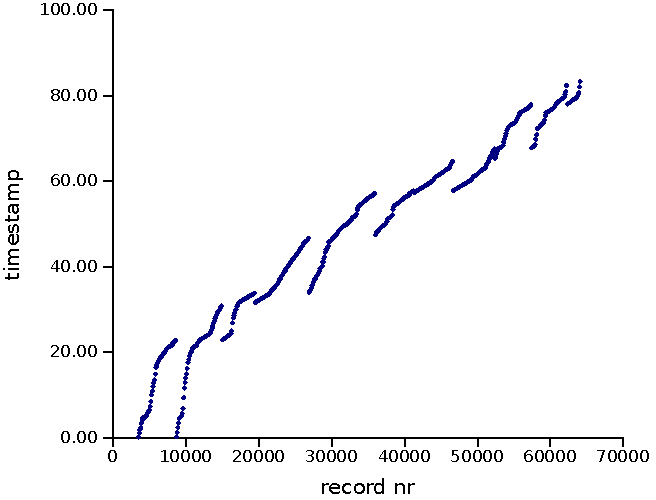
\includegraphics[scale=0.9]{res/timeRecord}
  \caption[Timestamp depending on the entry in the data file]{Timestamp depending on the entry in the data file. It was recorded on a two core system.  Only every 100th entry is shown. Timestamp is divided by $10^9$ and the start offset is subtracted. It can be seen that there exists a clear lower and upper bound for timestamps.\label{fig:timeRecord}}
\end{figure}

If one is only interested in processing the data from the data file, the callback functions can be used. After installed the callback functions, they are called with an occurrence of an record in the data file. As an example, \file{\textless perf source\textgreater /builtin-report.c} can be used.
